\chapter{Consultas de intervalo}

\index{range query}
\index{sum query}
\index{minimum query}
\index{maximum query}

Neste capítulo, discutimos estruturas de dados
que nos permitem processar eficientemente consultas de intervalo.
Em uma \key{consulta de intervalo},
nossa tarefa é calcular um valor
com base em um subvetor de um vetor.
Consultas de intervalo típicas são:
\begin{itemize}
\item $\texttt{soma}_q(a,b)$: calcular a soma dos valores no intervalo $[a,b]$
\item $\texttt{min}_q(a,b)$: encontrar o valor mínimo no intervalo $[a,b]$
\item $\texttt{max}_q(a,b)$: encontrar o valor máximo no intervalo $[a,b]$
\end{itemize}

Por exemplo, considere o intervalo $[3,6]$ no seguinte vetor:
\begin{center}
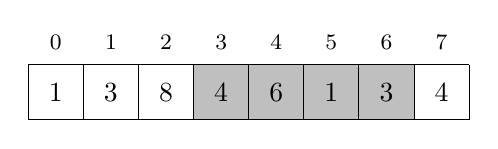
\begin{tikzpicture}[scale=0.7]
\fill[color=lightgray] (3,0) rectangle (7,1);
\draw (0,0) grid (8,1);

\node at (0.5,0.5) {$1$};
\node at (1.5,0.5) {$3$};
\node at (2.5,0.5) {$8$};
\node at (3.5,0.5) {$4$};
\node at (4.5,0.5) {$6$};
\node at (5.5,0.5) {$1$};
\node at (6.5,0.5) {$3$};
\node at (7.5,0.5) {$4$};

\footnotesize
\node at (0.5,1.4) {$0$};
\node at (1.5,1.4) {$1$};
\node at (2.5,1.4) {$2$};
\node at (3.5,1.4) {$3$};
\node at (4.5,1.4) {$4$};
\node at (5.5,1.4) {$5$};
\node at (6.5,1.4) {$6$};
\node at (7.5,1.4) {$7$};
\end{tikzpicture}
\end{center}
Neste caso, $\texttt{soma}_q(3,6)=14$,
$\texttt{min}_q(3,6)=1$ e $\texttt{max}_q(3,6)=6$.

Uma maneira simples de processar consultas de intervalo é usar
um loop que percorre todos os valores do vetor no intervalo.
Por exemplo, a seguinte função pode ser
usada para processar consultas de soma em um vetor:

\begin{lstlisting}
int sum(int a, int b) {
    int s = 0;
    for (int i = a; i <= b; i++) {
        s += array[i];
    }
    return s;
}
\end{lstlisting}

Esta função funciona em tempo $O(n)$,
onde $n$ é o tamanho do vetor.
Assim, podemos processar $q$ consultas em $O(nq)$
tempo usando a função.
No entanto, se $n$ e $q$ forem grandes, essa abordagem
é lenta. Felizmente, verifica-se que existem
maneiras de processar consultas de intervalo com muito mais eficiência.

\section{Consultas de vetor estático}

Primeiro, vamos nos concentrar em uma situação em que
o vetor é \emph{estático}, ou seja,
os valores do vetor nunca são atualizados entre as consultas.
Nesse caso, é suficiente construir
uma estrutura de dados estática que nos diga
a resposta para qualquer consulta possível.

\subsubsection{Consultas de soma}

\index{prefix sum array}

Podemos processar facilmente
consultas de soma em um vetor estático
construindo um \key{vetor de soma de prefixos}.
Cada valor no vetor de soma de prefixos é igual
à soma dos valores no vetor original até aquela posição,
ou seja, o valor na posição $k$ é $\texttt{soma}_q(0,k)$.
O vetor de soma de prefixos pode ser construído em tempo $O(n)$.

Por exemplo, considere o seguinte vetor:
\begin{center}
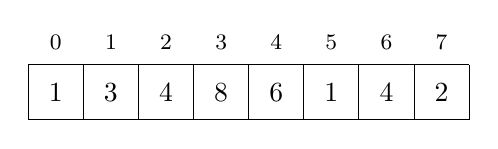
\begin{tikzpicture}[scale=0.7]
%\fill[color=lightgray] (3,0) rectangle (7,1);
\draw (0,0) grid (8,1);

\node at (0.5,0.5) {$1$};
\node at (1.5,0.5) {$3$};
\node at (2.5,0.5) {$4$};
\node at (3.5,0.5) {$8$};
\node at (4.5,0.5) {$6$};
\node at (5.5,0.5) {$1$};
\node at (6.5,0.5) {$4$};
\node at (7.5,0.5) {$2$};

\footnotesize
\node at (0.5,1.4) {$0$};
\node at (1.5,1.4) {$1$};
\node at (2.5,1.4) {$2$};
\node at (3.5,1.4) {$3$};
\node at (4.5,1.4) {$4$};
\node at (5.5,1.4) {$5$};
\node at (6.5,1.4) {$6$};
\node at (7.5,1.4) {$7$};
\end{tikzpicture}
\end{center}
O vetor de soma de prefixos correspondente é o seguinte:
\begin{center}
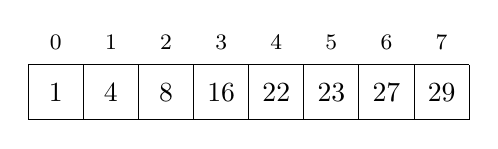
\begin{tikzpicture}[scale=0.7]
%\fill[color=lightgray] (3,0) rectangle (7,1);
\draw (0,0) grid (8,1);

\node at (0.5,0.5) {$1$};
\node at (1.5,0.5) {$4$};
\node at (2.5,0.5) {$8$};
\node at (3.5,0.5) {$16$};
\node at (4.5,0.5) {$22$};
\node at (5.5,0.5) {$23$};
\node at (6.5,0.5) {$27$};
\node at (7.5,0.5) {$29$};


\footnotesize
\node at (0.5,1.4) {$0$};
\node at (1.5,1.4) {$1$};
\node at (2.5,1.4) {$2$};
\node at (3.5,1.4) {$3$};
\node at (4.5,1.4) {$4$};
\node at (5.5,1.4) {$5$};
\node at (6.5,1.4) {$6$};
\node at (7.5,1.4) {$7$};
\end{tikzpicture}
\end{center}
Como o vetor de soma de prefixos contém todos os valores
de $\texttt{soma}_q(0,k)$,
podemos calcular qualquer valor de
$\texttt{soma}_q(a,b)$ em tempo $O(1)$ da seguinte forma:
\[ \texttt{soma}_q(a,b) = \texttt{soma}_q(0,b) - \texttt{soma}_q(0,a-1)\]
Ao definir $\texttt{soma}_q(0,-1)=0$,
a fórmula acima também é válida quando $a=0$.

Por exemplo, considere o intervalo $[3,6]$:
\begin{center}
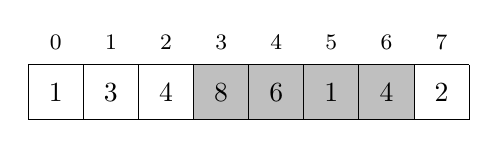
\begin{tikzpicture}[scale=0.7]
\fill[color=lightgray] (3,0) rectangle (7,1);
\draw (0,0) grid (8,1);

\node at (0.5,0.5) {$1$};
\node at (1.5,0.5) {$3$};
\node at (2.5,0.5) {$4$};
\node at (3.5,0.5) {$8$};
\node at (4.5,0.5) {$6$};
\node at (5.5,0.5) {$1$};
\node at (6.5,0.5) {$4$};
\node at (7.5,0.5) {$2$};

\footnotesize
\node at (0.5,1.4) {$0$};
\node at (1.5,1.4) {$1$};
\node at (2.5,1.4) {$2$};
\node at (3.5,1.4) {$3$};
\node at (4.5,1.4) {$4$};
\node at (5.5,1.4) {$5$};
\node at (6.5,1.4) {$6$};
\node at (7.5,1.4) {$7$};
\end{tikzpicture}
\end{center}
Nesse caso $\texttt{soma}_q(3,6)=8+6+1+4=19$.
Essa soma pode ser calculada a partir
de dois valores do vetor de soma de prefixos:
\begin{center}
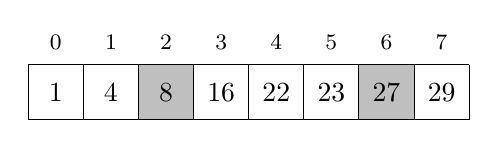
\begin{tikzpicture}[scale=0.7]
\fill[color=lightgray] (2,0) rectangle (3,1);
\fill[color=lightgray] (6,0) rectangle (7,1);
\draw (0,0) grid (8,1);

\node at (0.5,0.5) {$1$};
\node at (1.5,0.5) {$4$};
\node at (2.5,0.5) {$8$};
\node at (3.5,0.5) {$16$};
\node at (4.5,0.5) {$22$};
\node at (5.5,0.5) {$23$};
\node at (6.5,0.5) {$27$};
\node at (7.5,0.5) {$29$};

\footnotesize
\node at (0.5,1.4) {$0$};
\node at (1.5,1.4) {$1$};
\node at (2.5,1.4) {$2$};
\node at (3.5,1.4) {$3$};
\node at (4.5,1.4) {$4$};
\node at (5.5,1.4) {$5$};
\node at (6.5,1.4) {$6$};
\node at (7.5,1.4) {$7$};
\end{tikzpicture}
\end{center}
Assim, $\texttt{soma}_q(3,6)=\texttt{soma}_q(0,6)-\texttt{soma}_q(0,2)=27-8=19$.

Também é possível generalizar essa ideia
para dimensões superiores.
Por exemplo, podemos construir um vetor de soma de prefixos bidimensional que pode ser usado para calcular
a soma de qualquer subvetor retangular em tempo $O(1)$.
Cada soma em tal vetor corresponde a
um subvetor
que começa no canto superior esquerdo do vetor.

\begin{samepage}
A imagem a seguir ilustra a ideia:
\begin{center}
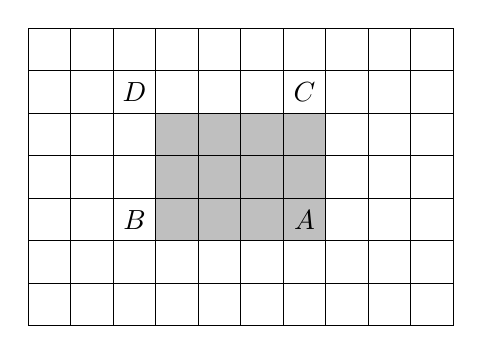
\begin{tikzpicture}[scale=0.54]
\draw[fill=lightgray] (3,2) rectangle (7,5);
\draw (0,0) grid (10,7);
\node[anchor=center] at (6.5, 2.5) {$A$};
\node[anchor=center] at (2.5, 2.5) {$B$};
\node[anchor=center] at (6.5, 5.5) {$C$};
\node[anchor=center] at (2.5, 5.5) {$D$};
\end{tikzpicture}
\end{center}
\end{samepage}

A soma do subvetor cinza pode ser calculada
usando a fórmula
\[S(A) - S(B) - S(C) + S(D),\]
onde $S(X)$ denota a soma dos valores
em um subvetor retangular
do canto superior esquerdo
até a posição de $X$.

\subsubsection{Consultas de mínimo}

\index{sparse table}

Consultas de mínimo são mais difíceis de processar
do que consultas de soma.
Ainda assim, existe um método de pré-processamento de $O(n \log n)$ bastante simples, após o qual podemos responder a qualquer consulta de mínimo
em tempo $O(1)$ \footnote {Esta técnica
foi introduzida em \cite{ben00} e às vezes
chamada de método \key{sparse table}.
Existem também técnicas mais sofisticadas \cite{fis06} onde
o tempo de pré-processamento é apenas $O(n)$, mas tais algoritmos
não são necessários em programação competitiva.}.
Observe que, como as consultas de mínimo e máximo podem
ser processadas de forma semelhante,
podemos nos concentrar nas consultas de mínimo.

A ideia é pré-calcular todos os valores de
$\textrm{min}_q(a,b)$ onde
$b-a+1$ (o comprimento do intervalo) é uma potência de dois.
Por exemplo, para o vetor

\begin{center}
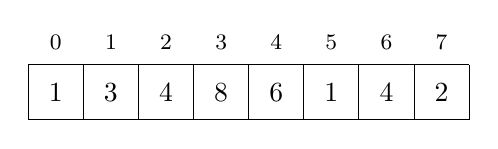
\begin{tikzpicture}[scale=0.7]
\draw (0,0) grid (8,1);

\node at (0.5,0.5) {$1$};
\node at (1.5,0.5) {$3$};
\node at (2.5,0.5) {$4$};
\node at (3.5,0.5) {$8$};
\node at (4.5,0.5) {$6$};
\node at (5.5,0.5) {$1$};
\node at (6.5,0.5) {$4$};
\node at (7.5,0.5) {$2$};

\footnotesize
\node at (0.5,1.4) {$0$};
\node at (1.5,1.4) {$1$};
\node at (2.5,1.4) {$2$};
\node at (3.5,1.4) {$3$};
\node at (4.5,1.4) {$4$};
\node at (5.5,1.4) {$5$};
\node at (6.5,1.4) {$6$};
\node at (7.5,1.4) {$7$};
\end{tikzpicture}
\end{center}
os seguintes valores são calculados:

\begin{center}
\begin{tabular}{ccc}

\begin{tabular}{lll}
$a$ & $b$ & $\texttt{min}_q(a,b)$ \\
\hline
0 & 0 & 1 \\
1 & 1 & 3 \\
2 & 2 & 4 \\
3 & 3 & 8 \\
4 & 4 & 6 \\
5 & 5 & 1 \\
6 & 6 & 4 \\
7 & 7 & 2 \\
\end{tabular}

&

\begin{tabular}{lll}
$a$ & $b$ & $\texttt{min}_q(a,b)$ \\
\hline
0 & 1 & 1 \\
1 & 2 & 3 \\
2 & 3 & 4 \\
3 & 4 & 6 \\
4 & 5 & 1 \\
5 & 6 & 1 \\
6 & 7 & 2 \\
\\
\end{tabular}

&

\begin{tabular}{lll}
$a$ & $b$ & $\texttt{min}_q(a,b)$ \\
\hline
0 & 3 & 1 \\
1 & 4 & 3 \\
2 & 5 & 1 \\
3 & 6 & 1 \\
4 & 7 & 1 \\
0 & 7 & 1 \\
\\
\\
\end{tabular}

\end{tabular}
\end{center}

O número de valores pré-calculados é $O(n \log n)$,
porque existem comprimentos de intervalo $O(\log n)$
que são potências de dois.
Os valores podem ser calculados de forma eficiente
usando a fórmula recursiva
\[\texttt{min}_q(a,b) = \min(\texttt{min}_q(a,a+w-1),\texttt{min}_q(a+w,b)),\]
onde $b-a+1$ é uma potência de dois e $w=(b-a+1)/2$.
Calcular todos esses valores leva tempo $O(n \log n)$.

Depois disso, qualquer valor de $\texttt{min}_q(a,b)$ pode ser calculado
em tempo $O(1)$ como um mínimo de dois valores pré-calculados.
Seja $k$ a maior potência de dois que não exceda $b-a+1$.
Podemos calcular o valor de $\texttt{min}_q(a,b)$ usando a fórmula
\[\texttt{min}_q(a,b) = \min(\texttt{min}_q(a,a+k-1),\texttt{min}_q(b-k+1,b)).\]
Na fórmula acima, o intervalo $[a,b]$ é representado
como a união dos intervalos $[a,a+k-1]$ e $[b-k+1,b]$, ambos de comprimento $k$.

Como exemplo, considere o intervalo $[1,6]$:
\begin{center}
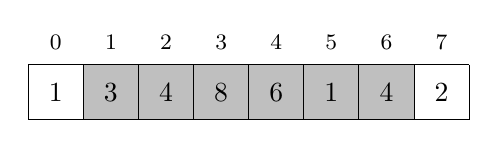
\begin{tikzpicture}[scale=0.7]
\fill[color=lightgray] (1,0) rectangle (7,1);
\draw (0,0) grid (8,1);

\node at (0.5,0.5) {$1$};
\node at (1.5,0.5) {$3$};
\node at (2.5,0.5) {$4$};
\node at (3.5,0.5) {$8$};
\node at (4.5,0.5) {$6$};
\node at (5.5,0.5) {$1$};
\node at (6.5,0.5) {$4$};
\node at (7.5,0.5) {$2$};

\footnotesize
\node at (0.5,1.4) {$0$};
\node at (1.5,1.4) {$1$};
\node at (2.5,1.4) {$2$};
\node at (3.5,1.4) {$3$};
\node at (4.5,1.4) {$4$};
\node at (5.5,1.4) {$5$};
\node at (6.5,1.4) {$6$};
\node at (7.5,1.4) {$7$};
\end{tikzpicture}
\end{center}
O comprimento do intervalo é 6,
e a maior potência de dois que
não excede 6 é 4.
Assim, o intervalo $[1,6]$ é
a união dos intervalos $[1,4]$ e $[3,6]$:
\begin{center}
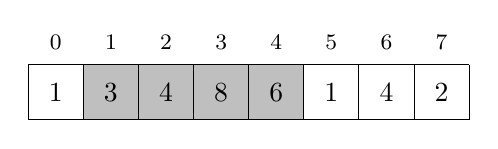
\begin{tikzpicture}[scale=0.7]
\fill[color=lightgray] (1,0) rectangle (5,1);
\draw (0,0) grid (8,1);

\node at (0.5,0.5) {$1$};
\node at (1.5,0.5) {$3$};
\node at (2.5,0.5) {$4$};
\node at (3.5,0.5) {$8$};
\node at (4.5,0.5) {$6$};
\node at (5.5,0.5) {$1$};
\node at (6.5,0.5) {$4$};
\node at (7.5,0.5) {$2$};

\footnotesize
\node at (0.5,1.4) {$0$};
\node at (1.5,1.4) {$1$};
\node at (2.5,1.4) {$2$};
\node at (3.5,1.4) {$3$};
\node at (4.5,1.4) {$4$};
\node at (5.5,1.4) {$5$};
\node at (6.5,1.4) {$6$};
\node at (7.5,1.4) {$7$};
\end{tikzpicture}
\end{center}
\begin{center}
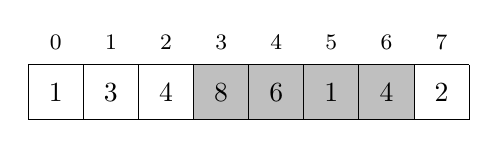
\begin{tikzpicture}[scale=0.7]
\fill[color=lightgray] (3,0) rectangle (7,1);
\draw (0,0) grid (8,1);

\node at (0.5,0.5) {$1$};
\node at (1.5,0.5) {$3$};
\node at (2.5,0.5) {$4$};
\node at (3.5,0.5) {$8$};
\node at (4.5,0.5) {$6$};
\node at (5.5,0.5) {$1$};
\node at (6.5,0.5) {$4$};
\node at (7.5,0.5) {$2$};


\footnotesize
\node at (0.5,1.4) {$0$};
\node at (1.5,1.4) {$1$};
\node at (2.5,1.4) {$2$};
\node at (3.5,1.4) {$3$};
\node at (4.5,1.4) {$4$};
\node at (5.5,1.4) {$5$};
\node at (6.5,1.4) {$6$};
\node at (7.5,1.4) {$7$};
\end{tikzpicture}
\end{center}
Como $\texttt{min}_q(1,4)=3$ e $\texttt{min}_q(3,6)=1$,
concluímos que $\texttt{min}_q(1,6)=1$.

\section{Árvore binária indexada}

\index{binary indexed tree}
\index{Fenwick tree}

Uma \key{árvore binária indexada} ou uma \key{árvore de Fenwick}\footnote{A
estrutura de árvore binária indexada foi apresentada por P. M. Fenwick em 1994 \cite{fen94}.}
pode ser vista como uma variante dinâmica de um vetor de soma de prefixos.
Ela suporta duas operações de tempo $O(\log n)$ em um vetor:
processar uma consulta de soma de intervalo e atualizar um valor.

A vantagem de uma árvore binária indexada é
que ela nos permite atualizar de forma eficiente
os valores do vetor entre as consultas de soma.
Isso não seria possível usando um vetor de soma de prefixos,
porque após cada atualização, seria necessário construir todo o
vetor de soma de prefixos novamente em tempo $O(n)$.

\subsubsection{Estrutura}

Mesmo que o nome da estrutura seja \emph{árvore} binária indexada,
ela é geralmente representada como um vetor.
Nesta seção, assumimos que todos os vetores são indexados a partir de um,
porque isso facilita a implementação.

Seja $p(k)$ a maior potência de dois que
divide $k$.
Armazenamos uma árvore binária indexada como um vetor \texttt{tree}
tal que
\[ \texttt{tree}[k] = \texttt{sum}_q(k-p(k)+1,k),\]
ou seja, cada posição $k$ contém a soma dos valores
em um intervalo do vetor original cujo comprimento é $p(k)$
e que termina na posição $k$.
Por exemplo, como $p(6)=2$, $\texttt{tree}[6]$
contém o valor de $\texttt{sum}_q(5,6)$.

Por exemplo, considere o seguinte vetor:
\begin{center}
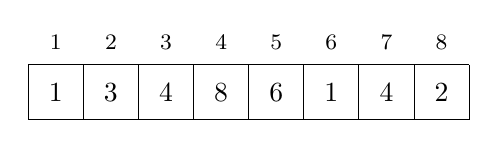
\begin{tikzpicture}[scale=0.7]
\draw (0,0) grid (8,1);

\node at (0.5,0.5) {$1$};
\node at (1.5,0.5) {$3$};
\node at (2.5,0.5) {$4$};
\node at (3.5,0.5) {$8$};
\node at (4.5,0.5) {$6$};
\node at (5.5,0.5) {$1$};
\node at (6.5,0.5) {$4$};
\node at (7.5,0.5) {$2$};

\footnotesize
\node at (0.5,1.4) {$1$};
\node at (1.5,1.4) {$2$};
\node at (2.5,1.4) {$3$};
\node at (3.5,1.4) {$4$};
\node at (4.5,1.4) {$5$};
\node at (5.5,1.4) {$6$};
\node at (6.5,1.4) {$7$};
\node at (7.5,1.4) {$8$};
\end{tikzpicture}
\end{center}

A árvore binária indexada correspondente é a seguinte:
\begin{center}
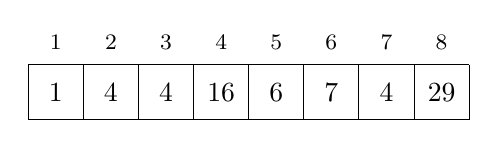
\begin{tikzpicture}[scale=0.7]
\draw (0,0) grid (8,1);

\node at (0.5,0.5) {$1$};
\node at (1.5,0.5) {$4$};
\node at (2.5,0.5) {$4$};
\node at (3.5,0.5) {$16$};
\node at (4.5,0.5) {$6$};
\node at (5.5,0.5) {$7$};
\node at (6.5,0.5) {$4$};
\node at (7.5,0.5) {$29$};

\footnotesize
\node at (0.5,1.4) {$1$};
\node at (1.5,1.4) {$2$};
\node at (2.5,1.4) {$3$};
\node at (3.5,1.4) {$4$};
\node at (4.5,1.4) {$5$};
\node at (5.5,1.4) {$6$};
\node at (6.5,1.4) {$7$};
\node at (7.5,1.4) {$8$};
\end{tikzpicture}
\end{center}

A figura a seguir mostra mais claramente
como cada valor na árvore binária indexada
corresponde a um intervalo no vetor original:

\begin{center}
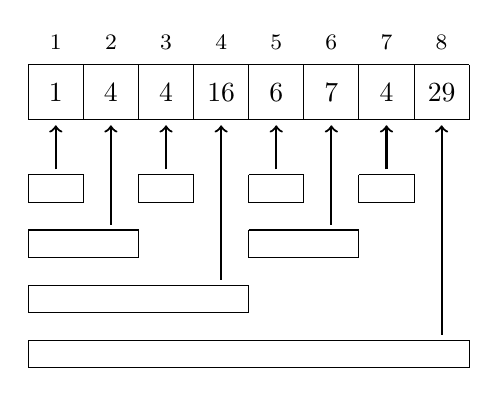
\begin{tikzpicture}[scale=0.7]
\draw (0,0) grid (8,1);

\node at (0.5,0.5) {$1$};
\node at (1.5,0.5) {$4$};
\node at (2.5,0.5) {$4$};
\node at (3.5,0.5) {$16$};
\node at (4.5,0.5) {$6$};
\node at (5.5,0.5) {$7$};
\node at (6.5,0.5) {$4$};
\node at (7.5,0.5) {$29$};

\footnotesize
\node at (0.5,1.4) {$1$};
\node at (1.5,1.4) {$2$};
\node at (2.5,1.4) {$3$};
\node at (3.5,1.4) {$4$};
\node at (4.5,1.4) {$5$};
\node at (5.5,1.4) {$6$};
\node at (6.5,1.4) {$7$};
\node at (7.5,1.4) {$8$};

\draw[->,thick] (0.5,-0.9) -- (0.5,-0.1);
\draw[->,thick] (2.5,-0.9) -- (2.5,-0.1);
\draw[->,thick] (4.5,-0.9) -- (4.5,-0.1);
\draw[->,thick] (6.5,-0.9) -- (6.5,-0.1);
\draw[->,thick] (1.5,-1.9) -- (1.5,-0.1);
\draw[->,thick] (5.5,-1.9) -- (5.5,-0.1);
\draw[->,thick] (3.5,-2.9) -- (3.5,-0.1);
\draw[->,thick] (7.5,-3.9) -- (7.5,-0.1);

\draw (0,-1) -- (1,-1) -- (1,-1.5) -- (0,-1.5) -- (0,-1);
\draw (2,-1) -- (3,-1) -- (3,-1.5) -- (2,-1.5) -- (2,-1);
\draw (4,-1) -- (5,-1) -- (5,-1.5) -- (4,-1.5) -- (4,-1);
\draw (6,-1) -- (7,-1) -- (7,-1.5) -- (6,-1.5) -- (6,-1);
\draw (0,-2) -- (2,-2) -- (2,-2.5) -- (0,-2.5) -- (0,-2);
\draw (4,-2) -- (6,-2) -- (6,-2.5) -- (4,-2.5) -- (4,-2);
\draw (0,-3) -- (4,-3) -- (4,-3.5) -- (0,-3.5) -- (0,-3);
\draw (0,-4) -- (8,-4) -- (8,-4.5) -- (0,-4.5) -- (0,-4);
\end{tikzpicture}
\end{center}

Usando uma árvore binária indexada,
qualquer valor de $\texttt{sum}_q(1,k)$
pode ser calculado em tempo $O(\log n)$,
porque um intervalo $[1,k]$ sempre pode ser dividido em
$O(\log n)$ intervalos cujas somas são armazenadas na árvore.

Por exemplo, o intervalo $[1,7]$ consiste
nos seguintes intervalos:
\begin{center}
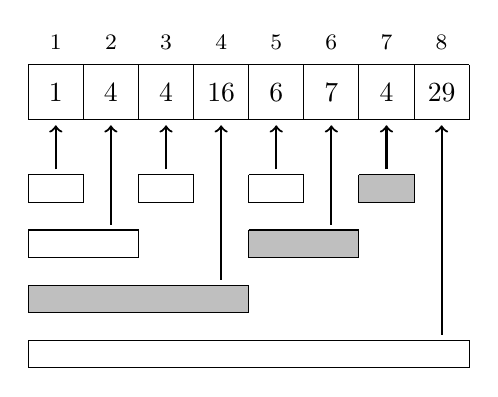
\begin{tikzpicture}[scale=0.7]
\draw (0,0) grid (8,1);

\node at (0.5,0.5) {$1$};
\node at (1.5,0.5) {$4$};
\node at (2.5,0.5) {$4$};
\node at (3.5,0.5) {$16$};
\node at (4.5,0.5) {$6$};
\node at (5.5,0.5) {$7$};
\node at (6.5,0.5) {$4$};
\node at (7.5,0.5) {$29$};

\footnotesize
\node at (0.5,1.4) {$1$};
\node at (1.5,1.4) {$2$};
\node at (2.5,1.4) {$3$};
\node at (3.5,1.4) {$4$};
\node at (4.5,1.4) {$5$};
\node at (5.5,1.4) {$6$};
\node at (6.5,1.4) {$7$};
\node at (7.5,1.4) {$8$};

\draw[->,thick] (0.5,-0.9) -- (0.5,-0.1);
\draw[->,thick] (2.5,-0.9) -- (2.5,-0.1);
\draw[->,thick] (4.5,-0.9) -- (4.5,-0.1);
\draw[->,thick] (6.5,-0.9) -- (6.5,-0.1);
\draw[->,thick] (1.5,-1.9) -- (1.5,-0.1);
\draw[->,thick] (5.5,-1.9) -- (5.5,-0.1);
\draw[->,thick] (3.5,-2.9) -- (3.5,-0.1);
\draw[->,thick] (7.5,-3.9) -- (7.5,-0.1);

\draw (0,-1) -- (1,-1) -- (1,-1.5) -- (0,-1.5) -- (0,-1);
\draw (2,-1) -- (3,-1) -- (3,-1.5) -- (2,-1.5) -- (2,-1);
\draw (4,-1) -- (5,-1) -- (5,-1.5) -- (4,-1.5) -- (4,-1);
\draw[fill=lightgray] (6,-1) -- (7,-1) -- (7,-1.5) -- (6,-1.5) -- (6,-1);
\draw (0,-2) -- (2,-2) -- (2,-2.5) -- (0,-2.5) -- (0,-2);
\draw[fill=lightgray] (4,-2) -- (6,-2) -- (6,-2.5) -- (4,-2.5) -- (4,-2);
\draw[fill=lightgray] (0,-3) -- (4,-3) -- (4,-3.5) -- (0,-3.5) -- (0,-3);
\draw (0,-4) -- (8,-4) -- (8,-4.5) -- (0,-4.5) -- (0,-4);
\end{tikzpicture}
\end{center}
Assim, podemos calcular a soma correspondente da seguinte forma:
\[\texttt{sum}_q(1,7)=\texttt{sum}_q(1,4)+\texttt{sum}_q(5,6)+\texttt{sum}_q(7,7)=16+7+4=27\]

Para calcular o valor de $\texttt{sum}_q(a,b)$ onde $a>1$,
podemos usar o mesmo truque que usamos com vetores de soma de prefixos:
\[ \texttt{sum}_q(a,b) = \texttt{sum}_q(1,b) - \texttt{sum}_q(1,a-1).\]
Como podemos calcular $\texttt{sum}_q(1,b)$
e $\texttt{sum}_q(1,a-1)$ em tempo $O(\log n)$,
a complexidade de tempo total é $O(\log n)$.

Então, após atualizar um valor no vetor original,
vários valores na árvore binária indexada
devem ser atualizados.
Por exemplo, se o valor na posição 3 mudar,
as somas dos seguintes intervalos mudam:
\begin{center}
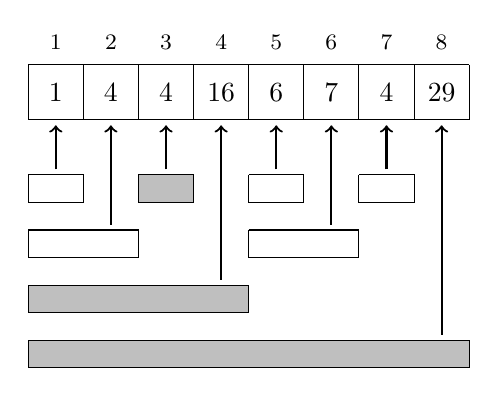
\begin{tikzpicture}[scale=0.7]
\draw (0,0) grid (8,1);

\node at (0.5,0.5) {$1$};
\node at (1.5,0.5) {$4$};
\node at (2.5,0.5) {$4$};
\node at (3.5,0.5) {$16$};
\node at (4.5,0.5) {$6$};
\node at (5.5,0.5) {$7$};
\node at (6.5,0.5) {$4$};
\node at (7.5,0.5) {$29$};

\footnotesize
\node at (0.5,1.4) {$1$};
\node at (1.5,1.4) {$2$};
\node at (2.5,1.4) {$3$};
\node at (3.5,1.4) {$4$};
\node at (4.5,1.4) {$5$};
\node at (5.5,1.4) {$6$};
\node at (6.5,1.4) {$7$};
\node at (7.5,1.4) {$8$};

\draw[->,thick] (0.5,-0.9) -- (0.5,-0.1);
\draw[->,thick] (2.5,-0.9) -- (2.5,-0.1);
\draw[->,thick] (4.5,-0.9) -- (4.5,-0.1);
\draw[->,thick] (6.5,-0.9) -- (6.5,-0.1);
\draw[->,thick] (1.5,-1.9) -- (1.5,-0.1);
\draw[->,thick] (5.5,-1.9) -- (5.5,-0.1);
\draw[->,thick] (3.5,-2.9) -- (3.5,-0.1);
\draw[->,thick] (7.5,-3.9) -- (7.5,-0.1);

\draw (0,-1) -- (1,-1) -- (1,-1.5) -- (0,-1.5) -- (0,-1);
\draw[fill=lightgray] (2,-1) -- (3,-1) -- (3,-1.5) -- (2,-1.5) -- (2,-1);
\draw (4,-1) -- (5,-1) -- (5,-1.5) -- (4,-1.5) -- (4,-1);
\draw (6,-1) -- (7,-1) -- (7,-1.5) -- (6,-1.5) -- (6,-1);
\draw (0,-2) -- (2,-2) -- (2,-2.5) -- (0,-2.5) -- (0,-2);
\draw (4,-2) -- (6,-2) -- (6,-2.5) -- (4,-2.5) -- (4,-2);
\draw[fill=lightgray] (0,-3) -- (4,-3) -- (4,-3.5) -- (0,-3.5) -- (0,-3);
\draw[fill=lightgray] (0,-4) -- (8,-4) -- (8,-4.5) -- (0,-4.5) -- (0,-4);
\end{tikzpicture}
\end{center}

Como cada elemento do vetor pertence a $O(\log n)$
intervalos na árvore binária indexada,
é suficiente atualizar $O(\log n)$ valores na árvore.

\subsubsection{Implementação}

As operações de uma árvore binária indexada podem ser
implementadas eficientemente usando operações de bits.
O fato chave necessário é que podemos
calcular qualquer valor de $p(k)$ usando a fórmula
\[p(k) = k \& -k.\]

A seguinte função calcula o valor de $\texttt{sum}_q(1,k)$:
\begin{lstlisting}
int sum(int k) {
    int s = 0;
    while (k >= 1) {
        s += tree[k];
        k -= k&-k;
    }
    return s;
}
\end{lstlisting}

A seguinte função aumenta o
valor do vetor na posição $k$ em $x$
($x$ pode ser positivo ou negativo):
\begin{lstlisting}
void add(int k, int x) {
    while (k <= n) {
        tree[k] += x;
        k += k&-k;
    }
}
\end{lstlisting}

A complexidade de tempo de ambas as funções é
$O(\log n)$, porque as funções acessam $O(\log n)$
valores na árvore binária indexada, e cada movimento
para a próxima posição leva tempo $O(1)$.

\section{Árvore de segmentos}

\index{segment tree}

Uma \key{árvore de segmentos}\footnote{A implementação bottom-up neste capítulo corresponde
àquela em \cite{sta06}. Estruturas semelhantes foram usadas
no final dos anos 1970 para resolver problemas geométricos \cite{ben80}.} é uma estrutura de dados
que suporta duas operações:
processar uma consulta de intervalo e
atualizar um valor do vetor.
As árvores de segmentos podem suportar
consultas de soma, consultas de mínimo e máximo e muitas outras
consultas para que ambas as operações funcionem em tempo $O(\log n)$.

Comparada a uma árvore binária indexada,
a vantagem de uma árvore de segmentos é que ela é
uma estrutura de dados mais geral.
Enquanto as árvores binárias indexadas suportam apenas
consultas de soma\footnote{Na verdade, usando \emph{duas} árvores binárias 
indexadas, é possível suportar consultas de mínimo \cite{dim15},
mas isso é mais complicado do que usar uma árvore de segmentos.},
as árvores de segmentos também suportam outras consultas.
Por outro lado, uma árvore de segmentos requer mais
memória e é um pouco mais difícil de implementar.

\subsubsection{Estrutura}

Uma árvore de segmentos é uma árvore binária
tal que os nós no nível inferior da árvore
correspondem aos elementos do vetor,
e os outros nós
contêm informações necessárias para processar consultas de intervalo.

Nesta seção, assumimos que o tamanho
do vetor é uma potência de dois e a indexação baseada em zero
é usada, porque é conveniente construir
uma árvore de segmentos para tal vetor.
Se o tamanho do vetor não for uma potência de dois,
podemos sempre anexar elementos extras a ele.

Vamos primeiro discutir árvores de segmentos que suportam consultas de soma.
Como exemplo, considere o seguinte vetor:
\begin{center}
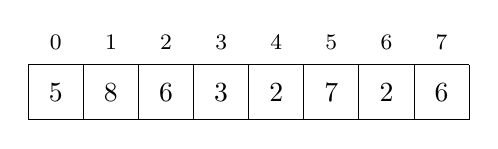
\begin{tikzpicture}[scale=0.7]
\draw (0,0) grid (8,1);

\node at (0.5,0.5) {$5$};
\node at (1.5,0.5) {$8$};
\node at (2.5,0.5) {$6$};
\node at (3.5,0.5) {$3$};
\node at (4.5,0.5) {$2$};
\node at (5.5,0.5) {$7$};
\node at (6.5,0.5) {$2$};
\node at (7.5,0.5) {$6$};

\footnotesize
\node at (0.5,1.4) {$0$};
\node at (1.5,1.4) {$1$};
\node at (2.5,1.4) {$2$};
\node at (3.5,1.4) {$3$};
\node at (4.5,1.4) {$4$};
\node at (5.5,1.4) {$5$};
\node at (6.5,1.4) {$6$};
\node at (7.5,1.4) {$7$};
\end{tikzpicture}
\end{center}
A árvore de segmentos correspondente é a seguinte:
\begin{center}
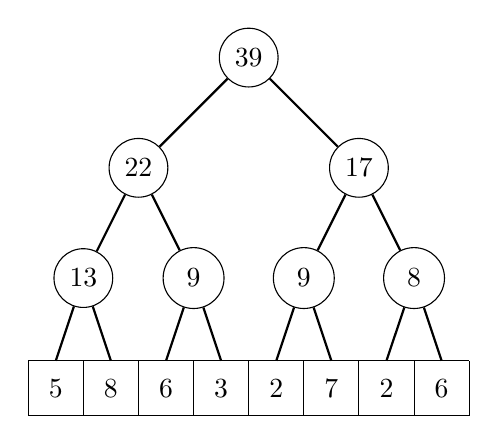
\begin{tikzpicture}[scale=0.7]
\draw (0,0) grid (8,1);

\node[anchor=center] at (0.5, 0.5) {5};
\node[anchor=center] at (1.5, 0.5) {8};
\node[anchor=center] at (2.5, 0.5) {6};
\node[anchor=center] at (3.5, 0.5) {3};
\node[anchor=center] at (4.5, 0.5) {2};
\node[anchor=center] at (5.5, 0.5) {7};
\node[anchor=center] at (6.5, 0.5) {2};
\node[anchor=center] at (7.5, 0.5) {6};

\node[draw, circle] (a) at (1,2.5) {13};
\path[draw,thick,-] (a) -- (0.5,1);
\path[draw,thick,-] (a) -- (1.5,1);
\node[draw, circle,minimum size=22pt] (b) at (3,2.5) {9};
\path[draw,thick,-] (b) -- (2.5,1);
\path[draw,thick,-] (b) -- (3.5,1);
\node[draw, circle,minimum size=22pt] (c) at (5,2.5) {9};
\path[draw,thick,-] (c) -- (4.5,1);
\path[draw,thick,-] (c) -- (5.5,1);
\node[draw, circle,minimum size=22pt] (d) at (7,2.5) {8};
\path[draw,thick,-] (d) -- (6.5,1);
\path[draw,thick,-] (d) -- (7.5,1);

\node[draw, circle] (i) at (2,4.5) {22};
\path[draw,thick,-] (i) -- (a);
\path[draw,thick,-] (i) -- (b);
\node[draw, circle] (j) at (6,4.5) {17};
\path[draw,thick,-] (j) -- (c);
\path[draw,thick,-] (j) -- (d);

\node[draw, circle] (m) at (4,6.5) {39};
\path[draw,thick,-] (m) -- (i);
\path[draw,thick,-] (m) -- (j);
\end{tikzpicture}
\end{center}

Cada nó interno da árvore
corresponde a um intervalo do vetor
cujo tamanho é uma potência de dois.
Na árvore acima, o valor de cada nó interno
é a soma dos valores correspondentes do vetor,
e pode ser calculado como a soma dos
valores de seu nó filho esquerdo e direito.

Acontece que qualquer intervalo $[a,b]$
pode ser dividido em $O(\log n)$ intervalos
cujos valores são armazenados nos nós da árvore.
Por exemplo, considere o intervalo [2,7]:
\begin{center}
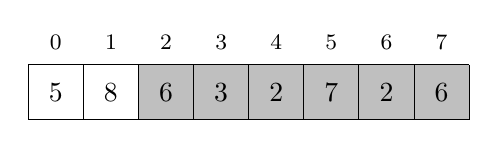
\begin{tikzpicture}[scale=0.7]
\fill[color=gray!50] (2,0) rectangle (8,1);
\draw (0,0) grid (8,1);

\node[anchor=center] at (0.5, 0.5) {5};
\node[anchor=center] at (1.5, 0.5) {8};
\node[anchor=center] at (2.5, 0.5) {6};
\node[anchor=center] at (3.5, 0.5) {3};
\node[anchor=center] at (4.5, 0.5) {2};
\node[anchor=center] at (5.5, 0.5) {7};
\node[anchor=center] at (6.5, 0.5) {2};
\node[anchor=center] at (7.5, 0.5) {6};

\footnotesize
\node at (0.5,1.4) {$0$};
\node at (1.5,1.4) {$1$};
\node at (2.5,1.4) {$2$};
\node at (3.5,1.4) {$3$};
\node at (4.5,1.4) {$4$};
\node at (5.5,1.4) {$5$};
\node at (6.5,1.4) {$6$};
\node at (7.5,1.4) {$7$};
\end{tikzpicture}
\end{center}
Aqui $\texttt{sum}_q(2,7)=6+3+2+7+2+6=26$.
Neste caso, os dois nós da árvore a seguir
correspondem ao intervalo:
\begin{center}
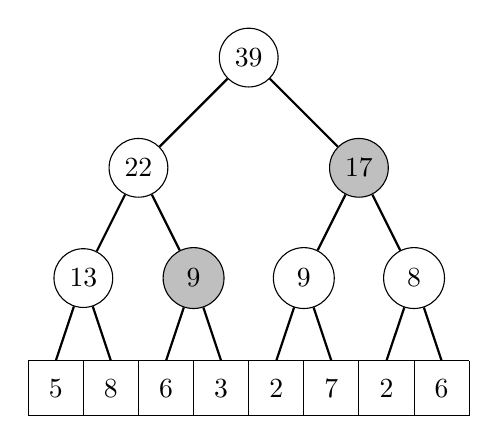
\begin{tikzpicture}[scale=0.7]
\draw (0,0) grid (8,1);

\node[anchor=center] at (0.5, 0.5) {5};
\node[anchor=center] at (1.5, 0.5) {8};
\node[anchor=center] at (2.5, 0.5) {6};
\node[anchor=center] at (3.5, 0.5) {3};
\node[anchor=center] at (4.5, 0.5) {2};
\node[anchor=center] at (5.5, 0.5) {7};
\node[anchor=center] at (6.5, 0.5) {2};
\node[anchor=center] at (7.5, 0.5) {6};

\node[draw, circle] (a) at (1,2.5) {13};
\path[draw,thick,-] (a) -- (0.5,1);
\path[draw,thick,-] (a) -- (1.5,1);
\node[draw, circle,fill=gray!50,minimum size=22pt] (b) at (3,2.5) {9};
\path[draw,thick,-] (b) -- (2.5,1);
\path[draw,thick,-] (b) -- (3.5,1);
\node[draw, circle,minimum size=22pt] (c) at (5,2.5) {9};
\path[draw,thick,-] (c) -- (4.5,1);
\path[draw,thick,-] (c) -- (5.5,1);
\node[draw, circle,minimum size=22pt] (d) at (7,2.5) {8};
\path[draw,thick,-] (d) -- (6.5,1);
\path[draw,thick,-] (d) -- (7.5,1);

\node[draw, circle] (i) at (2,4.5) {22};
\path[draw,thick,-] (i) -- (a);
\path[draw,thick,-] (i) -- (b);
\node[draw, circle,fill=gray!50] (j) at (6,4.5) {17};
\path[draw,thick,-] (j) -- (c);
\path[draw,thick,-] (j) -- (d);

\node[draw, circle] (m) at (4,6.5) {39};
\path[draw,thick,-] (m) -- (i);
\path[draw,thick,-] (m) -- (j);
\end{tikzpicture}
\end{center}
Assim, outra maneira de calcular a soma é $9+17=26$.

Quando a soma é calculada usando nós
localizados o mais alto possível na árvore,
no máximo dois nós em cada nível
da árvore são necessários.
Portanto, o número total de nós
é $O(\log n)$.

Após uma atualização do vetor,
devemos atualizar todos os nós
cujo valor depende do valor atualizado.
Isso pode ser feito percorrendo o caminho
do elemento do vetor atualizado até o nó superior
e atualizando os nós ao longo do caminho.

A figura a seguir mostra quais nós da árvore
mudam se o valor do vetor 7 mudar:

\begin{center}
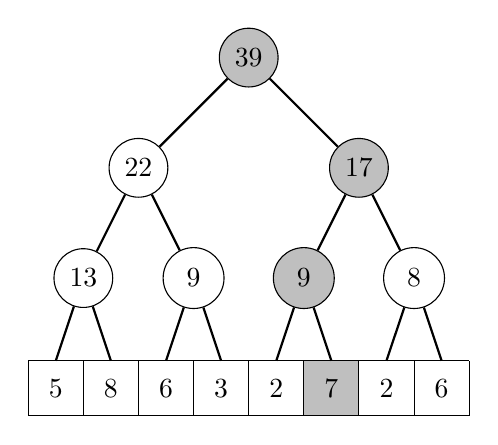
\begin{tikzpicture}[scale=0.7]
\fill[color=gray!50] (5,0) rectangle (6,1);
\draw (0,0) grid (8,1);

\node[anchor=center] at (0.5, 0.5) {5};
\node[anchor=center] at (1.5, 0.5) {8};
\node[anchor=center] at (2.5, 0.5) {6};
\node[anchor=center] at (3.5, 0.5) {3};
\node[anchor=center] at (4.5, 0.5) {2};
\node[anchor=center] at (5.5, 0.5) {7};
\node[anchor=center] at (6.5, 0.5) {2};
\node[anchor=center] at (7.5, 0.5) {6};

\node[draw, circle] (a) at (1,2.5) {13};
\path[draw,thick,-] (a) -- (0.5,1);
\path[draw,thick,-] (a) -- (1.5,1);
\node[draw, circle,minimum size=22pt] (b) at (3,2.5) {9};
\path[draw,thick,-] (b) -- (2.5,1);
\path[draw,thick,-] (b) -- (3.5,1);
\node[draw, circle,minimum size=22pt,fill=gray!50] (c) at (5,2.5) {9};
\path[draw,thick,-] (c) -- (4.5,1);
\path[draw,thick,-] (c) -- (5.5,1);
\node[draw, circle,minimum size=22pt] (d) at (7,2.5) {8};
\path[draw,thick,-] (d) -- (6.5,1);
\path[draw,thick,-] (d) -- (7.5,1);

\node[draw, circle] (i) at (2,4.5) {22};
\path[draw,thick,-] (i) -- (a);
\path[draw,thick,-] (i) -- (b);
\node[draw, circle,fill=gray!50] (j) at (6,4.5) {17};
\path[draw,thick,-] (j) -- (c);
\path[draw,thick,-] (j) -- (d);

\node[draw, circle,fill=gray!50] (m) at (4,6.5) {39};
\path[draw,thick,-] (m) -- (i);
\path[draw,thick,-] (m) -- (j);
\end{tikzpicture}
\end{center}

O caminho de baixo para cima
sempre consiste em $O(\log n)$ nós,
então cada atualização muda $O(\log n)$ nós na árvore.

\subsubsection{Implementação}

Armazenamos uma árvore de segmentos como um vetor
de $2n$ elementos, onde $n$ é o tamanho do
vetor original e uma potência de dois.
Os nós da árvore são armazenados de cima para baixo:
$\texttt{tree}[1]$ é o nó superior,
$\texttt{tree}[2]$ e $\texttt{tree}[3]$
são seus filhos, e assim por diante.
Finalmente, os valores de $\texttt{tree}[n]$
a $\texttt{tree}[2n-1]$ correspondem aos
valores do vetor original
no nível inferior da árvore.

Por exemplo, a árvore de segmentos
\begin{center}
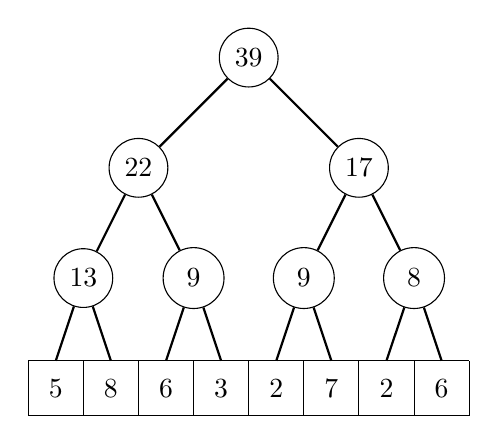
\begin{tikzpicture}[scale=0.7]
\draw (0,0) grid (8,1);

\node[anchor=center] at (0.5, 0.5) {5};
\node[anchor=center] at (1.5, 0.5) {8};
\node[anchor=center] at (2.5, 0.5) {6};
\node[anchor=center] at (3.5, 0.5) {3};
\node[anchor=center] at (4.5, 0.5) {2};
\node[anchor=center] at (5.5, 0.5) {7};
\node[anchor=center] at (6.5, 0.5) {2};
\node[anchor=center] at (7.5, 0.5) {6};

\node[draw, circle] (a) at (1,2.5) {13};
\path[draw,thick,-] (a) -- (0.5,1);
\path[draw,thick,-] (a) -- (1.5,1);
\node[draw, circle,minimum size=22pt] (b) at (3,2.5) {9};
\path[draw,thick,-] (b) -- (2.5,1);
\path[draw,thick,-] (b) -- (3.5,1);
\node[draw, circle,minimum size=22pt] (c) at (5,2.5) {9};
\path[draw,thick,-] (c) -- (4.5,1);
\path[draw,thick,-] (c) -- (5.5,1);
\node[draw, circle,minimum size=22pt] (d) at (7,2.5) {8};
\path[draw,thick,-] (d) -- (6.5,1);
\path[draw,thick,-] (d) -- (7.5,1);

\node[draw, circle] (i) at (2,4.5) {22};
\path[draw,thick,-] (i) -- (a);
\path[draw,thick,-] (i) -- (b);
\node[draw, circle] (j) at (6,4.5) {17};
\path[draw,thick,-] (j) -- (c);
\path[draw,thick,-] (j) -- (d);

\node[draw, circle] (m) at (4,6.5) {39};
\path[draw,thick,-] (m) -- (i);
\path[draw,thick,-] (m) -- (j);
\end{tikzpicture}
\end{center}
é armazenada da seguinte forma:
\begin{center}
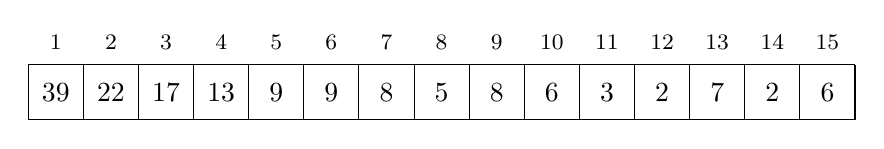
\begin{tikzpicture}[scale=0.7]
\draw (0,0) grid (15,1);

\node at (0.5,0.5) {$39$};
\node at (1.5,0.5) {$22$};
\node at (2.5,0.5) {$17$};
\node at (3.5,0.5) {$13$};
\node at (4.5,0.5) {$9$};
\node at (5.5,0.5) {$9$};
\node at (6.5,0.5) {$8$};
\node at (7.5,0.5) {$5$};
\node at (8.5,0.5) {$8$};
\node at (9.5,0.5) {$6$};
\node at (10.5,0.5) {$3$};
\node at (11.5,0.5) {$2$};
\node at (12.5,0.5) {$7$};
\node at (13.5,0.5) {$2$};
\node at (14.5,0.5) {$6$};

\footnotesize
\node at (0.5,1.4) {$1$};
\node at (1.5,1.4) {$2$};
\node at (2.5,1.4) {$3$};
\node at (3.5,1.4) {$4$};
\node at (4.5,1.4) {$5$};
\node at (5.5,1.4) {$6$};
\node at (6.5,1.4) {$7$};
\node at (7.5,1.4) {$8$};
\node at (8.5,1.4) {$9$};
\node at (9.5,1.4) {$10$};
\node at (10.5,1.4) {$11$};
\node at (11.5,1.4) {$12$};
\node at (12.5,1.4) {$13$};
\node at (13.5,1.4) {$14$};
\node at (14.5,1.4) {$15$};
\end{tikzpicture}
\end{center}
Usando essa representação,
o pai de $\texttt{tree}[k]$
é $\texttt{tree}[\lfloor k/2 \rfloor]$,
e seus filhos são $\texttt{tree}[2k]$
e $\texttt{tree}[2k+1]$.
Note que isso implica que a posição de um nó
é par se for um filho esquerdo e ímpar se for um filho direito.

A seguinte função
calcula o valor de $\texttt{sum}_q(a,b)$:
\begin{lstlisting}
int sum(int a, int b) {
    a += n; b += n;
    int s = 0;
    while (a <= b) {
        if (a%2 == 1) s += tree[a++];
        if (b%2 == 0) s += tree[b--];
        a /= 2; b /= 2;
    }
    return s;
}
\end{lstlisting}
A função mantém um intervalo
que é inicialmente $[a+n,b+n]$.
Então, a cada passo, o intervalo é movido
um nível mais alto na árvore,
e antes disso, os valores dos nós que não
pertencem ao intervalo superior são adicionados à soma.

A seguinte função aumenta o valor do vetor
na posição $k$ por $x$:
\begin{lstlisting}
void add(int k, int x) {
    k += n;
    tree[k] += x;
    for (k /= 2; k >= 1; k /= 2) {
        tree[k] = tree[2*k]+tree[2*k+1];
    }
}
\end{lstlisting}
Primeiro a função atualiza o valor
no nível inferior da árvore.
Depois disso, a função atualiza os valores de todos
os nós internos da árvore, até que alcance
o nó superior da árvore.

Ambas as funções acima funcionam
em tempo $O(\log n)$, pois uma árvore de segmentos
de $n$ elementos consiste em $O(\log n)$ níveis,
e as funções movem um nível mais alto
na árvore a cada passo.

\subsubsection{Outras consultas}

Árvores de segmentos podem suportar todas as consultas de intervalo
onde é possível dividir um intervalo em duas partes,
calcular a resposta separadamente para ambas as partes
e então combinar as respostas de forma eficiente.
Exemplos de tais consultas são
mínimo e máximo, maior divisor comum,
e operações de bits and, or e xor.

Por exemplo, a seguinte árvore de segmentos
suporta consultas de mínimo:

\begin{center}
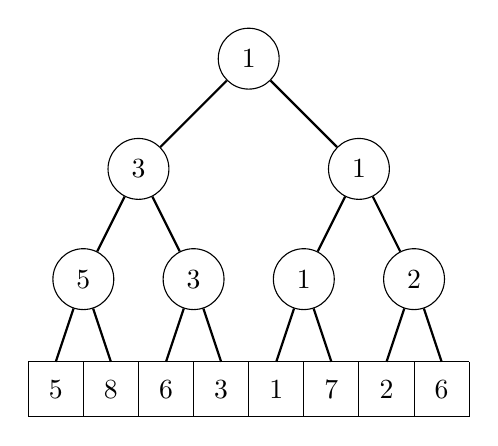
\begin{tikzpicture}[scale=0.7]
\draw (0,0) grid (8,1);

\node[anchor=center] at (0.5, 0.5) {5};
\node[anchor=center] at (1.5, 0.5) {8};
\node[anchor=center] at (2.5, 0.5) {6};
\node[anchor=center] at (3.5, 0.5) {3};
\node[anchor=center] at (4.5, 0.5) {1};
\node[anchor=center] at (5.5, 0.5) {7};
\node[anchor=center] at (6.5, 0.5) {2};
\node[anchor=center] at (7.5, 0.5) {6};

\node[draw, circle,minimum size=22pt] (a) at (1,2.5) {5};
\path[draw,thick,-] (a) -- (0.5,1);
\path[draw,thick,-] (a) -- (1.5,1);
\node[draw, circle,minimum size=22pt] (b) at (3,2.5) {3};
\path[draw,thick,-] (b) -- (2.5,1);
\path[draw,thick,-] (b) -- (3.5,1);
\node[draw, circle,minimum size=22pt] (c) at (5,2.5) {1};
\path[draw,thick,-] (c) -- (4.5,1);
\path[draw,thick,-] (c) -- (5.5,1);
\node[draw, circle,minimum size=22pt] (d) at (7,2.5) {2};
\path[draw,thick,-] (d) -- (6.5,1);
\path[draw,thick,-] (d) -- (7.5,1);

\node[draw, circle,minimum size=22pt] (i) at (2,4.5) {3};
\path[draw,thick,-] (i) -- (a);
\path[draw,thick,-] (i) -- (b);
\node[draw, circle,minimum size=22pt] (j) at (6,4.5) {1};
\path[draw,thick,-] (j) -- (c);
\path[draw,thick,-] (j) -- (d);

\node[draw, circle,minimum size=22pt] (m) at (4,6.5) {1};
\path[draw,thick,-] (m) -- (i);
\path[draw,thick,-] (m) -- (j);
\end{tikzpicture}
\end{center}

Neste caso, cada nó da árvore contém
o menor valor no intervalo do vetor correspondente.
O nó superior da árvore contém o menor
valor em todo o vetor.
As operações podem ser implementadas como anteriormente,
mas em vez de somas, os mínimos são calculados.

A estrutura de uma árvore de segmentos também nos permite
usar a busca binária para localizar elementos do vetor.
Por exemplo, se a árvore suporta consultas de mínimo,
podemos encontrar a posição de um elemento
com o menor valor em $O(\log n)$ tempo.

Por exemplo, na árvore acima, um
elemento com o menor valor 1 pode ser encontrado
traversando um caminho para baixo a partir do nó superior:

\begin{center}
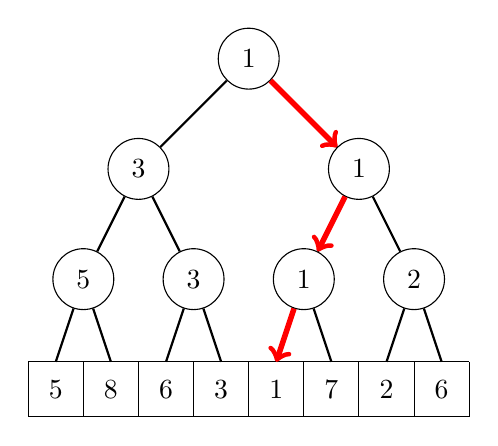
\begin{tikzpicture}[scale=0.7]
\draw (0,0) grid (8,1);

\node[anchor=center] at (0.5, 0.5) {5};
\node[anchor=center] at (1.5, 0.5) {8};
\node[anchor=center] at (2.5, 0.5) {6};
\node[anchor=center] at (3.5, 0.5) {3};
\node[anchor=center] at (4.5, 0.5) {1};
\node[anchor=center] at (5.5, 0.5) {7};
\node[anchor=center] at (6.5, 0.5) {2};
\node[anchor=center] at (7.5, 0.5) {6};

\node[draw, circle,minimum size=22pt] (a) at (1,2.5) {5};
\path[draw,thick,-] (a) -- (0.5,1);
\path[draw,thick,-] (a) -- (1.5,1);
\node[draw, circle,minimum size=22pt] (b) at (3,2.5) {3};
\path[draw,thick,-] (b) -- (2.5,1);
\path[draw,thick,-] (b) -- (3.5,1);
\node[draw, circle,minimum size=22pt] (c) at (5,2.5) {1};
\path[draw,thick,-] (c) -- (4.5,1);
\path[draw,thick,-] (c) -- (5.5,1);
\node[draw, circle,minimum size=22pt] (d) at (7,2.5) {2};
\path[draw,thick,-] (d) -- (6.5,1);
\path[draw,thick,-] (d) -- (7.5,1);

\node[draw, circle,minimum size=22pt] (i) at (2,4.5) {3};
\path[draw,thick,-] (i) -- (a);
\path[draw,thick,-] (i) -- (b);
\node[draw, circle,minimum size=22pt] (j) at (6,4.5) {1};
\path[draw,thick,-] (j) -- (c);
\path[draw,thick,-] (j) -- (d);

\node[draw, circle,minimum size=22pt] (m) at (4,6.5) {1};
\path[draw,thick,-] (m) -- (i);
\path[draw,thick,-] (m) -- (j);

\path[draw=red,thick,->,line width=2pt] (m) -- (j);
\path[draw=red,thick,->,line width=2pt] (j) -- (c);
\path[draw=red,thick,->,line width=2pt] (c) -- (4.5,1);
\end{tikzpicture}
\end{center}

\section{Técnicas adicionais}

\subsubsection{Compressão de índices}

Uma limitação em estruturas de dados que
são construídas sobre um vetor é que
os elementos são indexados usando
inteiros consecutivos.
Dificuldades surgem quando índices grandes
são necessários.
Por exemplo, se desejarmos usar o índice $10^9$,
o vetor deve conter $10^9$
elementos, o que exigiria muita memória.

\index{compressão de índices}

No entanto, geralmente podemos contornar essa limitação
usando \key{compressão de índices},
onde os índices originais são substituídos
por índices $1,2,3,$ etc.
Isso pode ser feito se soubermos todos os índices
necessários durante o algoritmo antecipadamente.

A ideia é substituir cada índice original $x$
por $c(x)$, onde $c$ é uma função que
comprime os índices.
Exigimos que a ordem dos índices
não mude, então se $a<b$, então $c(a)<c(b)$.
Isso nos permite realizar consultas convenientemente
mesmo que os índices sejam comprimidos.

Por exemplo, se os índices originais são
$555$, $10^9$ e $8$, os novos índices são:

\[
\begin{array}{lcl}
c(8) & = & 1 \\
c(555) & = & 2 \\
c(10^9) & = & 3 \\
\end{array}
\]

\subsubsection{Atualizações de intervalo}

Até agora, implementamos estruturas de dados
que suportam consultas de intervalo e atualizações
de valores únicos.
Vamos agora considerar uma situação oposta,
onde devemos atualizar intervalos e
recuperar valores únicos.
Vamos focar numa operação que aumenta todos
os elementos num intervalo $[a,b]$ por $x$.

\index{vetor de diferenças}

Surpreendentemente, podemos usar as estruturas de dados
apresentadas neste capítulo também nesta situação.
Para fazer isso, construímos um \key{vetor de diferenças}
cujos valores indicam
as diferenças entre valores consecutivos
no vetor original.
Assim, o vetor original é o
vetor de soma de prefixo do
vetor de diferenças.
Por exemplo, considere o seguinte vetor:

\begin{center}
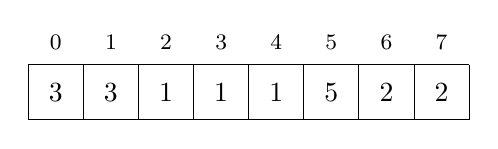
\begin{tikzpicture}[scale=0.7]
\draw (0,0) grid (8,1);

\node at (0.5,0.5) {$3$};
\node at (1.5,0.5) {$3$};
\node at (2.5,0.5) {$1$};
\node at (3.5,0.5) {$1$};
\node at (4.5,0.5) {$1$};
\node at (5.5,0.5) {$5$};
\node at (6.5,0.5) {$2$};
\node at (7.5,0.5) {$2$};


\footnotesize
\node at (0.5,1.4) {$0$};
\node at (1.5,1.4) {$1$};
\node at (2.5,1.4) {$2$};
\node at (3.5,1.4) {$3$};
\node at (4.5,1.4) {$4$};
\node at (5.5,1.4) {$5$};
\node at (6.5,1.4) {$6$};
\node at (7.5,1.4) {$7$};
\end{tikzpicture}
\end{center}

O vetor de diferenças para o vetor acima é o seguinte:
\begin{center}
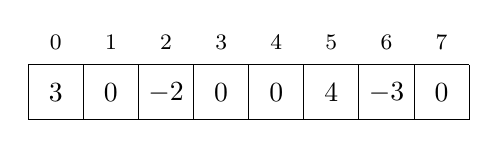
\begin{tikzpicture}[scale=0.7]
\draw (0,0) grid (8,1);

\node at (0.5,0.5) {$3$};
\node at (1.5,0.5) {$0$};
\node at (2.5,0.5) {$-2$};
\node at (3.5,0.5) {$0$};
\node at (4.5,0.5) {$0$};
\node at (5.5,0.5) {$4$};
\node at (6.5,0.5) {$-3$};
\node at (7.5,0.5) {$0$};


\footnotesize
\node at (0.5,1.4) {$0$};
\node at (1.5,1.4) {$1$};
\node at (2.5,1.4) {$2$};
\node at (3.5,1.4) {$3$};
\node at (4.5,1.4) {$4$};
\node at (5.5,1.4) {$5$};
\node at (6.5,1.4) {$6$};
\node at (7.5,1.4) {$7$};
\end{tikzpicture}
\end{center}

Por exemplo, o valor 2 na posição 6 no vetor original
corresponde à soma $3-2+4-3=2$ no vetor de diferenças.

A vantagem do vetor de diferenças é
que podemos atualizar um intervalo
no vetor original mudando apenas
dois elementos no vetor de diferenças.
Por exemplo, se quisermos
aumentar o vetor original
valores entre as posições 1 e 4 por 5,
basta aumentar o
valor do vetor de diferenças na posição 1 por 5
e diminuir o valor na posição 5 por 5.
O resultado é o seguinte:

\begin{center}
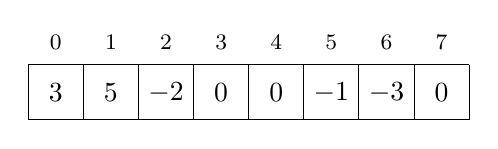
\begin{tikzpicture}[scale=0.7]
\draw (0,0) grid (8,1);

\node at (0.5,0.5) {$3$};
\node at (1.5,0.5) {$5$};
\node at (2.5,0.5) {$-2$};
\node at (3.5,0.5) {$0$};
\node at (4.5,0.5) {$0$};
\node at (5.5,0.5) {$-1$};
\node at (6.5,0.5) {$-3$};
\node at (7.5,0.5) {$0$};

\footnotesize
\node at (0.5,1.4) {$0$};
\node at (1.5,1.4) {$1$};
\node at (2.5,1.4) {$2$};
\node at (3.5,1.4) {$3$};
\node at (4.5,1.4) {$4$};
\node at (5.5,1.4) {$5$};
\node at (6.5,1.4) {$6$};
\node at (7.5,1.4) {$7$};
\end{tikzpicture}
\end{center}

De forma mais geral, para aumentar os valores
no intervalo $[a,b]$ por $x$,
aumentamos o valor na posição $a$ por $x$
e diminuímos o valor na posição $b+1$ por $x$.
Assim, é só necessário atualizar valores únicos
e processar consultas de soma,
para que possamos usar uma árvore binária indexada ou uma árvore de segmentos.

Um problema mais difícil é suportar tanto
consultas de intervalo quanto atualizações de intervalo.
No Capítulo 28 veremos que mesmo isso é possível.





